\begin{appendices}
  \addtocontents{toc}{\protect\setcounter{tocdepth}{1}}
    \makeatletter
    \addtocontents{toc}{%
      \begingroup
      \let\protect\l@chapter\protect\l@section
      \let\protect\l@section\protect\l@subsection
    }
    \makeatother

    \chapter{User Manual}
      \section{First section}
      \section{Second section}

    \chapter{Maintenance Manual\label{app:maintain}}
      \section{First section}
      \section{Second section}

    \chapter{Discussion Graph Representation\label{app:disc_graph}}
      \begin{figure}[h]
        \caption{A sample graph representation of the abortion discussion}
        \centering
        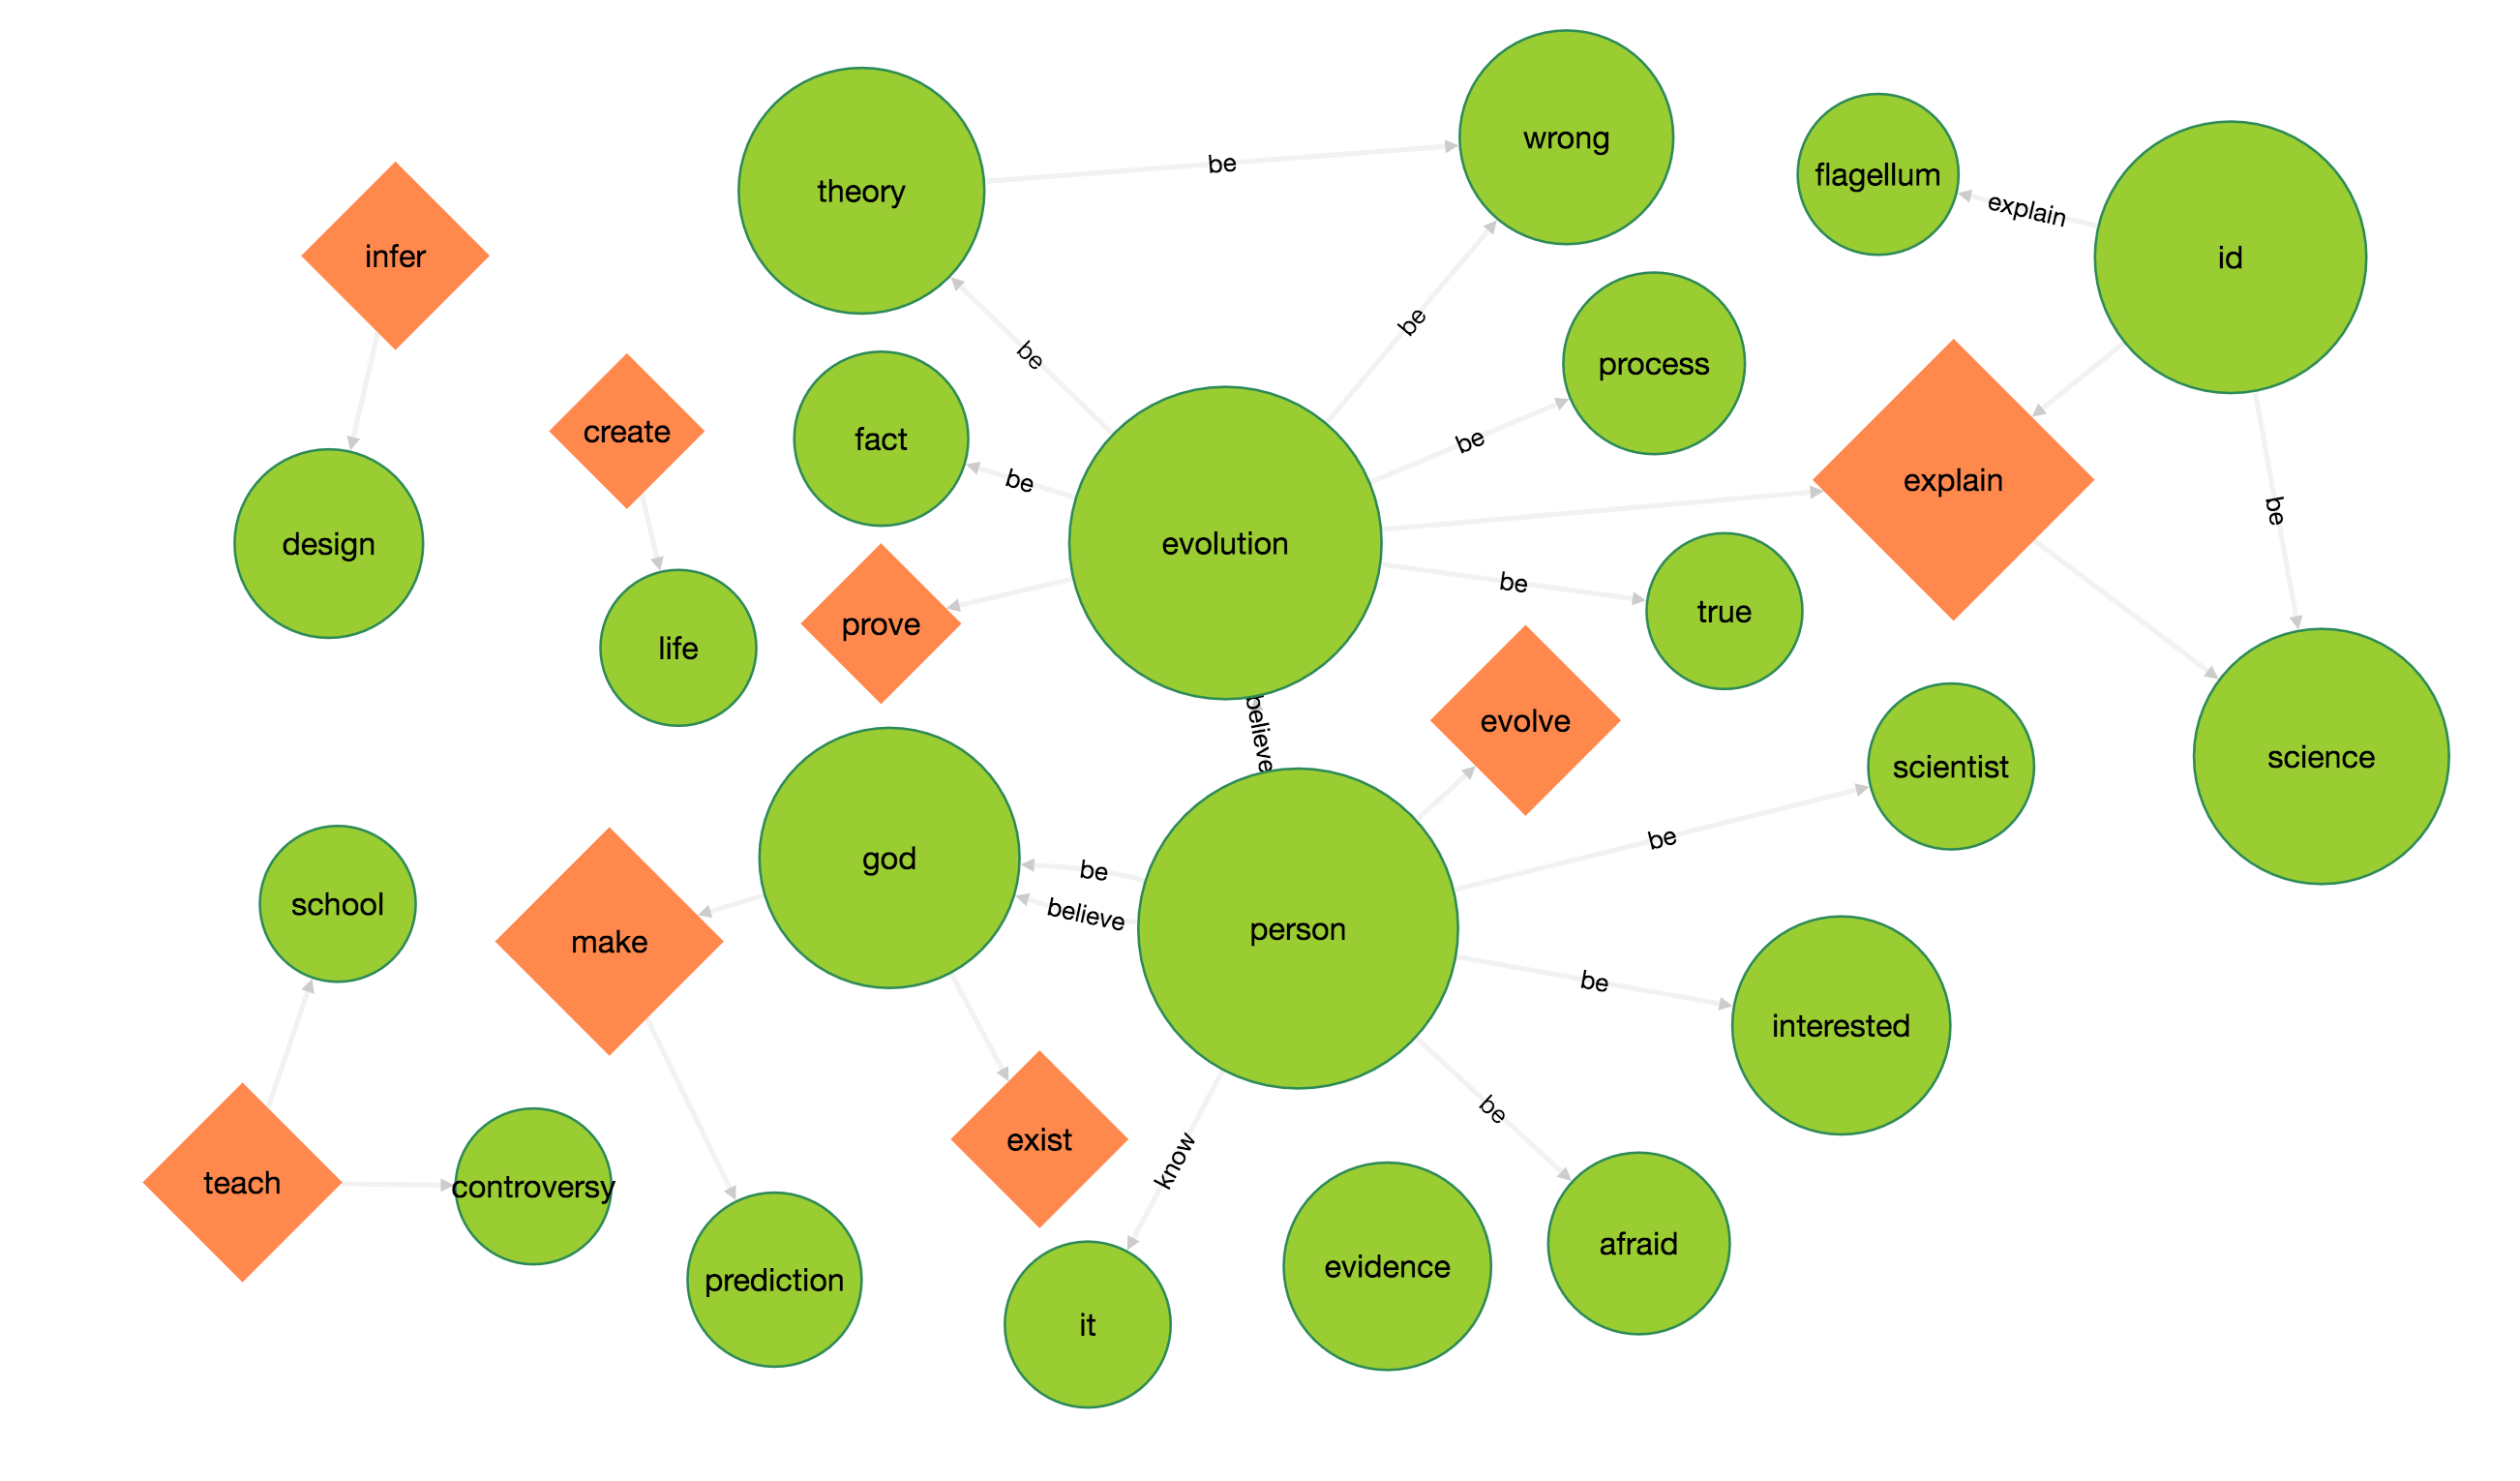
\includegraphics[width=0.8\textwidth]{disc_graph}
      \end{figure}

    \chapter{Blacklists\label{app:blacklists}}
      \section{Ambiguous subjects}
        \textit{it, that, this, which, what}

      \section{Disallowed Person Actions}
        The following verbs are not allowed in a 2 component point with a \texttt{PERSON.nsubj}:

        \textit{agree, argue, ask, begin, believe, believe, call, care, change, close, come, come, continue, debate, disagree, end, explain, fail, feel, feel, find, follow, get, go, go, guess, happen, hear, leave, live, lose, make, move, object, open, read, realize, refer, show, sit, speak, stand, start, support, take, talk, tell, think, try, understand, wonder, write}

      \section{Disallowed Points}
        \texttt{PERSON.nsubj be.verb} cannot be completed by: \textit{able, aware, correct, false, favor, glad, good, here, interested, likely, one, right, say, sorry, sure, true, willing, wrong}

        \noindent\texttt{PERSON.nsubj want.verb} cannot be completed by: \textit{have, what, what do}

        \noindent\texttt{PERSON.nsubj} cannot be completed by: \textit{say.verb what.dobj, mean.verb what.dobj, know.verb what.dobj, believe.verb what.dobj, see.verb what.dobj, see.verb argument.dobj, have.verb problem.dobj, tell.verb they.dobj, think.verb what.dobj, argue.verb in.prep fact.dobj, argue.verb with.prep you.dobj}

        \begin{itemize}
		  \item{debate.nsubj be.verb about.dobj}
		  \item{question.nsubj be.verb}
		  \item{make.verb claim.dobj}
		  \item{ask.verb yourself.dobj}
		  \item{thing.nsubj happen.verb}
		  \item{something.nsubj happen.verb}
        \end{itemize}

    \chapter{Summary Comparison Survey Section\label{app:survey-section}}
      \begin{figure}[h]
        \caption{An example study 1 survey section comparing a plain and stock survey.}
        \centering
        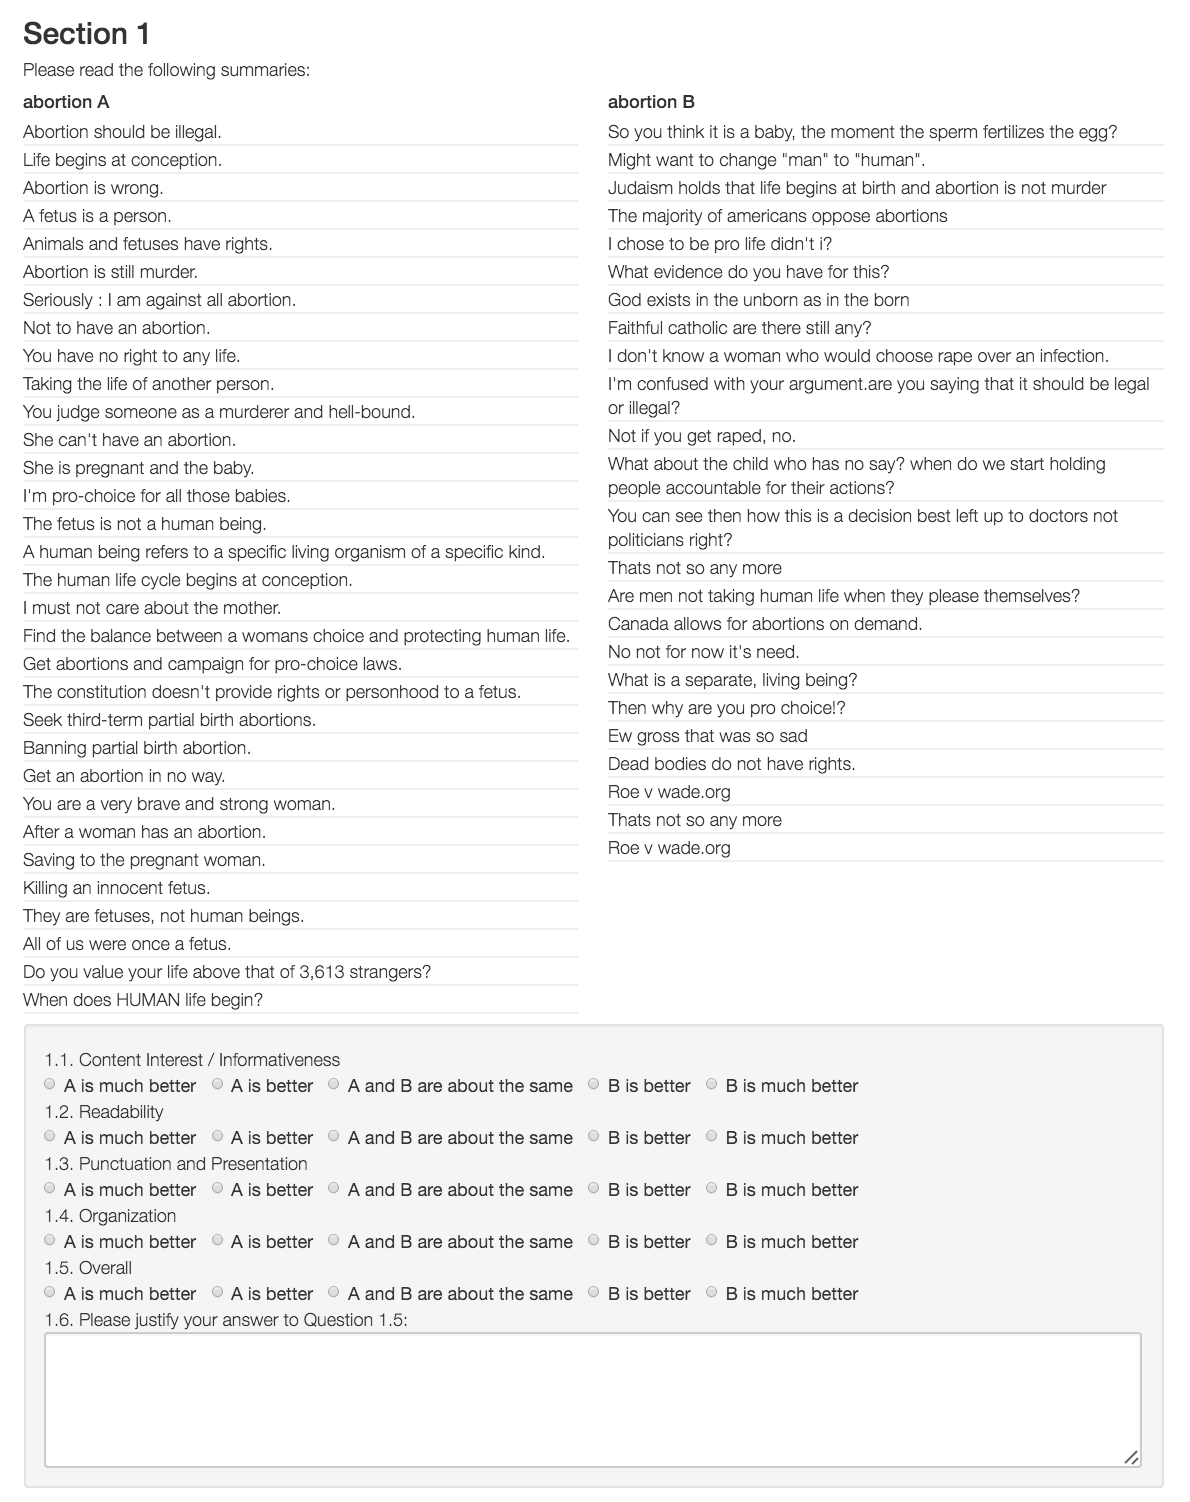
\includegraphics[width=0.9\textwidth]{survey}
      \end{figure}

    \chapter{Extract Survey Section\label{app:extract-survey-section}}
      \begin{figure}[h]
        \caption{An example study 2 survey section where participants rated extracts.}
        \centering
        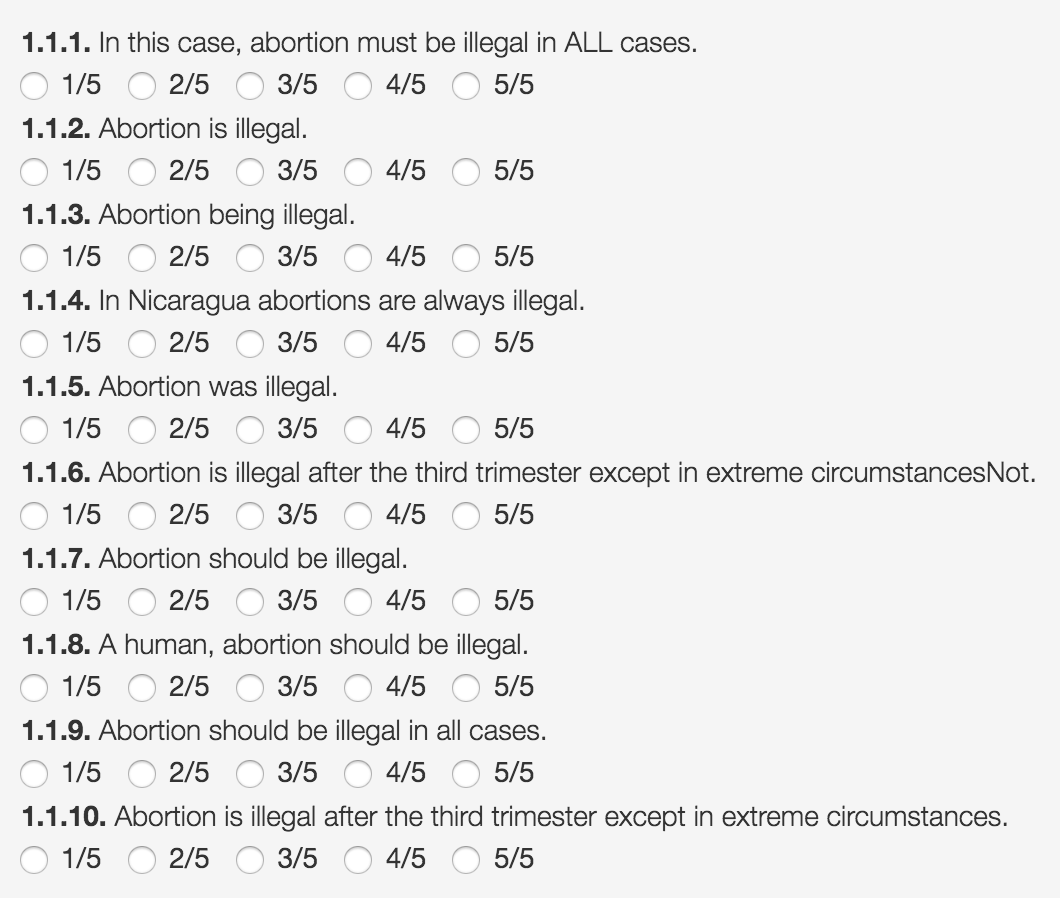
\includegraphics[width=0.9\textwidth]{survey2}
      \end{figure}

    \chapter{Evaluation Questionnaire Structure \label{app:evaluation-questionnaire-layouts}}
      \TBox[fill=red!15]{13cm}{
        \large Study 1 Questionnaire ($\times$6 variations in Latin Square) \\
        \normalsize
        \TBox[fill=black!1]{12.7cm}{
          \textbf{Section 1} Plain vs. Stock \\
          \small Order switches (3$\times$ Plain/Stock, 3$\times$ Stock/Plain)
          \normalsize

          \TBox[fill=white]{6cm}{
            Plain Summary (Topic A)
          }
          \TBox[fill=white]{6cm}{
            Stock Summary (Topic A)
          }
          \TBoxDash[fill=black!15]{12.4cm}{
            \textit{4 factor ratings; overall rating \& free text comment}
          }
        }
        \TBox[fill=black!1]{12.7cm}{
          \textbf{Section 2} Layout vs. Stock \\
          \small Order switches (3$\times$ Layout/Stock, 3$\times$ Stock/Layout)
          \normalsize

          \TBox[fill=white]{6cm}{
            Layout Summary (Topic \textbf{B})
          }
          \TBox[fill=white]{6cm}{
            Stock Summary (Topic \textbf{B})
          }
          \TBoxDash[fill=black!15]{12.4cm}{
            \textit{4 factor ratings; overall rating \& free text comment}
          }
        }
        \TBox[fill=black!1]{12.7cm}{
          \textbf{Section 3} Layout vs. Formatted \\
          \small Order switches (3$\times$ Layout/Formatted, 3$\times$ Form./Lay.)

          \small Summaries share content, only differ in formatting

          \small Layout summary reused from Section 2
          \normalsize

          \TBox[fill=white]{6cm}{
            Layout Summary (Topic \textbf{B})
          }
          \TBox[fill=white]{6cm}{
            Formatted Summ. (Topic \textbf{B})
          }
          \TBoxDash[fill=black!15]{12.4cm}{
            \textit{Overall rating only \& free text comment}
          }
        }
      }

      \vspace{2mm}
      \noindent\TBox[fill=green!15]{13cm}{
        \large Study 2 Questionnaire ($\times$6 variations) \\
        \normalsize
        \TBox[fill=black!1]{12.7cm}{
          \textbf{Section 1} Rating Extracts \\
          \normalsize

          \TBox[fill=white]{12.4cm}{
            Extract Set (Topic A) \textbf{($\times$3)}
            \TBoxDash[fill=black!15]{12.1cm}{
              \textit{Rating 1/5 per extract (approx. 10 extracts)}
            }
          }
        }
        \TBox[fill=black!1]{12.7cm}{
          \textbf{Section 2} Bigram vs. Random \\

          \TBox[fill=white]{6cm}{
            Bigram Summary (Topic A)
          }
          \TBox[fill=white]{6cm}{
            Random Summary (Topic A)
          }
          \TBoxDash[fill=black!15]{12.4cm}{
            \textit{Overall rating only \& free text comment}
          }
        }
      }

      \vspace{2mm}
      \noindent\TBox[fill=blue!15]{13cm}{
        \large Study 3 Questionnaire ($\times$2 variations each, $\times$6 variations total) \\
        \normalsize
        Participants had \textbf{two sheets}, each with different topics.
        \TBox[fill=black!1]{12.7cm}{
          \textbf{Section 1} Layout vs. Stock \\

          \TBox[fill=white]{6cm}{
            Layout Summary (Topic A)
          }
          \TBox[fill=white]{6cm}{
            Stock Summary (Topic A)
          }
          \TBoxDash[fill=black!15]{12.4cm}{
            \textit{Free text comments only}
          }
        }
      }

  \addtocontents{toc}{\endgroup}
\end{appendices}
